


\subsubsection{Verificação de Assinatura}
\paragraph{Mensagens de 256 bytes}

A Figura~\ref{fig:BENCHFINAL_VERIFY256_TIME} e a Tabela~\ref{tab:BENCHFINAL_VERIFY256_TIME} apresentam os resultados de tempo de CPU líquido para a operação de verificação de assinaturas com mensagens de 256 bytes. Diferentemente das etapas anteriores, em que as variações entre execuções foram praticamente desprezíveis, esta operação, por ser consideravelmente mais rápida, apresentou desvios padrão mais altos. Ainda assim, os valores permanecem dentro de uma faixa estável e aceitável, sem impacto significativo na análise comparativa.

Entre os esquemas clássicos, ambos os algoritmos mantiveram excelente desempenho, com o RSA apresentando, desta vez, um desempenho ligeiramente superior ao do ECDSA. Já entre os algoritmos pós-quânticos, todas as variantes de ML-DSA e Falcon apresentaram tempos de verificação competitivos e bastante próximos entre si, sendo cerca de uma vez e meia mais lentos que os esquemas clássicos.

Por outro lado, o SPHINCS+ continuou exibindo tempos consideravelmente maiores em todas as suas variantes. Um comportamento interessante observado nesta operação foi a inversão de tendência: as variantes \textit{f-simple}, otimizadas para reduzir o tempo de geração da assinatura, apresentaram desempenho inferior às \textit{s-simple}, voltadas à redução do tamanho das assinaturas. Isso ocorre porque, na verificação, o tamanho da assinatura tem maior influência sobre o tempo total de execução, fazendo com que as versões \textit{f}, que geram assinaturas maiores, apresentem custo mais elevado nessa etapa.

Ao comparar as duas plataformas, nota-se que o padrão geral se mantém, com o Raspberry Pi 3B exibindo tempos cerca de uma ordem de grandeza maiores que os do Ubuntu. No entanto, uma diferença relevante foi observada quanto às famílias de hash: no Ubuntu, as variantes SHA2 e SHAKE apresentaram resultados bastante próximos, com o SHA2 sendo levemente mais lento, comportamento inverso ao visto nas etapas de geração e assinatura. No Raspberry Pi, o SHA2 manteve-se como a opção mais custosa, mas com uma diferença ainda mais acentuada em relação ao SHAKE. 


\begin{figure}[h!]
    \centering
    \begin{subfigure}{1\textwidth}
        \includegraphics[width=\textwidth,frame]{Figures/ANALISEBENCHMARKFINAL/TEMPO/VERIFY/UBUNTU/bench_verify_256_cpu_net.png}
        \caption{Notebook Ubuntu}
    \end{subfigure}
    \par\vspace{1em}
    \begin{subfigure}{1\textwidth}
        \includegraphics[width=\textwidth,frame]{Figures/ANALISEBENCHMARKFINAL/TEMPO/VERIFY/PI/bench_verify_256_cpu_net.png}
        \caption{Raspberry Pi 3B}
    \end{subfigure}
    \caption{Comparação dos resultados de verificação com mensagem de 256 bytes}
    \label{fig:BENCHFINAL_VERIFY256_TIME}
\end{figure}

\begin{table}[h!]
\centering
\begin{tabularx}{\textwidth}{|Y||C|C||C|C|}
\hline
\multirow{2}{*}{\textbf{Algoritmo}} &
\multicolumn{2}{c||}{\textbf{Notebook Ubuntu}} &
\multicolumn{2}{c|}{\textbf{Raspberry Pi 3B}} \\ \cline{2-5}
& \textbf{Média} & \textbf{Desvio} & \textbf{Média} & \textbf{Desvio} \\
\Xhline{1pt}
sphincsshake256ssimple & 1.867 & 0.061 & 14.221 & 0.453 \\ \hline
sphincsshake256fsimple & 2.898 & 0.077 & 24.378 & 0.422 \\ \hline
sphincsshake192ssimple & 1.472 & 0.075 & 10.996 & 0.514 \\ \hline
sphincsshake192fsimple & 2.845 & 0.085 & 23.409 & 0.412 \\
\Xhline{1pt}
sphincsshake128ssimple & 1.300 & 0.083 & 8.799  & 0.406 \\ \hline
sphincsshake128fsimple & 2.319 & 0.078 & 17.666 & 0.564 \\ \hline
sphincssha2256ssimple  & 2.392 & 0.075 & 24.728 & 0.506 \\ \hline
sphincssha2256fsimple  & 3.002 & 0.083 & 39.279 & 0.523 \\
\Xhline{1pt}
sphincssha2192ssimple  & 2.179 & 0.078 & 20.307 & 0.410 \\ \hline
sphincssha2192fsimple  & 3.009 & 0.083 & 38.419 & 0.593 \\ \hline
sphincssha2128ssimple  & 1.925 & 0.076 & 16.716 & 0.584 \\ \hline
sphincssha2128fsimple  & 2.455 & 0.074 & 29.128 & 0.510 \\
\Xhline{1pt}
mldsa87   & 0.907 & 0.080 & 6.415 & 0.432 \\ \hline
mldsa65   & 0.854 & 0.075 & 5.585 & 0.542 \\ \hline
mldsa44   & 0.881 & 0.074 & 5.471 & 0.564 \\
\Xhline{1pt}
falcon512  & 0.889 & 0.071 & 5.476 & 0.560 \\ \hline
falcon1024 & 0.940 & 0.078 & 5.384 & 0.522 \\
\Xhline{1pt}
RSA & 0.538 & 0.073 & 3.551 & 0.532 \\ \hline
EC  & 0.681 & 0.069 & 4.012 & 0.565 \\ \hline
\end{tabularx}
\vspace{0.5em}
\caption{Comparação dos resultados de verificação com mensagem de 256 bytes}
\label{tab:BENCHFINAL_VERIFY256_TIME}
\end{table}


\paragraph{Mensagens de 100MB}

A Figura~\ref{fig:BENCHFINAL_VERIFY100MB_TIME} e a Tabela~\ref{tab:BENCHFINAL_VERIFY100MB_TIME} apresentam os resultados de verificação de assinaturas para mensagens de 100 MB. Entre os esquemas clássicos, RSA e ECDSA voltaram a apresentar os melhores tempos, com desempenhos praticamente equivalentes entre si. 

Entre os esquemas pós-quânticos, ML-DSA e Falcon mantiveram tempos muito próximos entre si em todas as variantes, mas desta vez situaram-se entre os algoritmos mais lentos, juntamente com todas as variantes SHAKE do SPHINCS+. 

Em contraste, as variantes SHA2-192 e SHA2-256 do SPHINCS+ apresentaram desempenho intermediário, sendo mais rápidas que as variantes SHAKE do SPHINCS+, ML-DSA e Falcon em ambas as plataformas.

Nas instâncias SHA2-128 do SPHINCS+, entretanto, observou-se uma diferença de comportamento entre as plataformas: no Ubuntu, essas variantes obtiveram tempos inferiores aos de todos os demais esquemas pós-quânticos, ficando atrás apenas dos algoritmos clássicos. Já no Raspberry Pi, apresentaram desempenho equivalente ao de ML-DSA, Falcon e SPHINCS+–SHAKE, posicionando-se entre os mais lentos.

Ao comparar as duas plataformas, nota-se que, diferentemente das etapas anteriores, a diferença de desempenho entre o Raspberry Pi e o ambiente Ubuntu não chegou a uma ordem de grandeza. Ainda assim, a distância relativa entre algoritmos clássicos e pós-quânticos permaneceu mais acentuada no Ubuntu, variando entre duas e cinco vezes, enquanto no Raspberry Pi os tempos ficaram mais próximos, com diferença máxima de aproximadamente uma vez e meia.

Por fim, comparando com os resultados obtidos para mensagens de 256 bytes, observa-se que o aumento do tamanho da mensagem novamente reduziu a disparidade entre os algoritmos, tornando os tempos de execução mais uniformes, especialmente na plataforma embarcada. Esse comportamento reforça que, em mensagens extensas, o custo computacional da verificação tende a ser dominado pelo processamento de dados, diminuindo o impacto relativo das diferenças estruturais entre os esquemas criptográficos.


\begin{figure}[h!]
    \centering
    \begin{subfigure}{1\textwidth}
        \includegraphics[width=\textwidth,frame]{Figures/ANALISEBENCHMARKFINAL/TEMPO/VERIFY/UBUNTU/bench_verify_100000000_cpu_net.png}
        \caption{Notebook Ubuntu}
    \end{subfigure}
    \par\vspace{1em}
    \begin{subfigure}{1\textwidth}
        \includegraphics[width=\textwidth,frame]{Figures/ANALISEBENCHMARKFINAL/TEMPO/VERIFY/PI/bench_verify_100000000_cpu_net.png}
        \caption{Raspberry Pi 3B}
    \end{subfigure}
    \caption{Comparação dos resultados de verificação com mensagem de 100MB}
    \label{fig:BENCHFINAL_VERIFY100MB_TIME}
\end{figure}

\begin{table}[h!]
\centering
\begin{tabularx}{\textwidth}{|Y||C|C||C|C|}
\hline
\multirow{2}{*}{\textbf{Algoritmo}} &
\multicolumn{2}{c||}{\textbf{Notebook Ubuntu}} &
\multicolumn{2}{c|}{\textbf{Raspberry Pi 3B}} \\ \cline{2-5}
& \textbf{Média} & \textbf{Desvio} & \textbf{Média} & \textbf{Desvio} \\
\Xhline{1pt}
sphincsshake256ssimple & 496.466 & 0.363 & 1676.828 & 1.838 \\ \hline
sphincsshake256fsimple & 497.612 & 0.388 & 1685.871 & 2.086 \\ \hline
sphincsshake192ssimple & 496.212 & 0.298 & 1673.929 & 2.016 \\ \hline
sphincsshake192fsimple & 497.703 & 0.328 & 1686.847 & 1.910 \\
\Xhline{1pt}
sphincsshake128ssimple & 495.590 & 0.324 & 1671.733 & 2.078 \\ \hline
sphincsshake128fsimple & 496.531 & 0.371 & 1683.209 & 1.991 \\ \hline
sphincssha2256ssimple  & 324.539 & 0.420 & 1337.329 & 2.376 \\ \hline
sphincssha2256fsimple  & 325.081 & 0.327 & 1352.857 & 1.680 \\
\Xhline{1pt}
sphincssha2192ssimple  & 324.884 & 0.358 & 1336.238 & 1.927 \\ \hline
sphincssha2192fsimple  & 325.646 & 0.359 & 1353.407 & 2.211 \\ \hline
sphincssha2128ssimple  & 208.349 & 0.367 & 1711.234 & 1.819 \\ \hline
sphincssha2128fsimple  & 208.696 & 0.330 & 1723.437 & 1.805 \\
\Xhline{1pt}
mldsa87   & 495.116 & 0.357 & 1670.748 & 2.047 \\ \hline
mldsa65   & 495.543 & 0.356 & 1670.921 & 1.691 \\ \hline
mldsa44   & 495.097 & 0.361 & 1670.853 & 1.945 \\
\Xhline{1pt}
falcon512  & 494.991 & 0.360 & 1672.710 & 1.960 \\ \hline
falcon1024 & 494.630 & 0.425 & 1670.388 & 2.015 \\
\Xhline{1pt}
RSA & 90.256 & 0.262 & 1094.009 & 0.968 \\ \hline
EC  & 90.281 & 0.278 & 1094.847 & 0.948 \\ \hline
\end{tabularx}
\vspace{0.5em}
\caption{Comparação dos resultados de verificação com mensagem de 100MB}
\label{tab:BENCHFINAL_VERIFY100MB_TIME}
\end{table}








\subsubsection{Ciclo Completo}
\paragraph{Mensagens de 256 bytes}

A Figura~\ref{fig:BENCHFINAL_ALL256_TIME} e a Tabela~\ref{tab:BENCHFINAL_ALL256_TIME} apresentam os resultados do ciclo completo, que representa a soma das três operações — geração de chaves, assinatura e verificação — executadas sequencialmente. Entre os esquemas clássicos, o ECDSA manteve-se como o mais eficiente entre todos os algoritmos, enquanto o RSA apresentou um dos maiores tempos do conjunto, superando inclusive a maioria dos esquemas pós-quânticos, com exceção das variantes \textit{s-simple} do SPHINCS+. Essa diferença é explicada principalmente pelo custo de geração de chaves, operação em que o RSA se mostrou significativamente mais custoso, apesar de seu ótimo desempenho nas etapas de assinatura e verificação.

Entre os algoritmos pós-quânticos, o ML-DSA apresentou o melhor desempenho geral, com tempos próximos aos do ECDSA — cerca de 1,5 vez mais lentos — e desempenho consistentemente equilibrado entre as três operações. O Falcon, que havia demonstrado resultados equivalentes ao ML-DSA nas etapas individuais de assinatura e verificação, apresentou um leve aumento no tempo total devido ao custo de geração de chaves, mas ainda se manteve entre os esquemas mais rápidos do conjunto.

As variantes \textit{f-simple} do SPHINCS+ exibiram desempenho intermediário, sendo substancialmente mais lentas que ML-DSA, Falcon e ECDSA, mas ainda abaixo dos tempos do RSA e das variantes \textit{s-simple}. Estas últimas, voltadas à economia de tamanho de assinatura, apresentaram novamente os maiores tempos de execução, com desempenho bastante inferior ao dos demais esquemas. Assim como observado nas etapas anteriores, manteve-se o padrão curioso em que as variantes de nível 192 mostraram-se mais lentas que as de nível 256.

A comparação entre plataformas revela comportamento consistente: o Raspberry Pi 3B apresentou tempos cerca de uma ordem de grandeza superiores aos observados no Ubuntu, mantendo, porém, as mesmas relações de desempenho entre algoritmos. Também se repetiu o padrão identificado nas demais operações, em que as variantes SHAKE foram mais lentas no Ubuntu, enquanto as SHA apresentaram maiores custos no Raspberry Pi, possivelmente em razão de diferenças nas otimizações das bibliotecas de hash entre arquiteturas x86-64 e ARM.

Por fim, é importante destacar que o tempo total do ciclo completo não reflete diretamente o custo típico de uso dos algoritmos em aplicações reais, já que a geração de chaves é uma operação muito menos frequente que assinatura e verificação. Assim, o grande tempo total observado no RSA ou a diferença entre Falcon e ML-DSA são ampliados pela inclusão de uma etapa que, na prática, teria impacto marginal no desempenho global de um sistema.


\begin{figure}[h!]
    \centering
    \begin{subfigure}{1\textwidth}
        \includegraphics[width=\textwidth,frame]{Figures/ANALISEBENCHMARKFINAL/TEMPO/ALL/UBUNTU/bench_all_256_cpu_net.png}
        \caption{Notebook Ubuntu}
    \end{subfigure}
    \par\vspace{1em}
    \begin{subfigure}{1\textwidth}
        \includegraphics[width=\textwidth,frame]{Figures/ANALISEBENCHMARKFINAL/TEMPO/ALL/PI/bench_all_256_cpu_net.png}
        \caption{Raspberry Pi 3B}
    \end{subfigure}
    \caption{Comparação dos resultados do ciclo completo com mensagem de 256 bytes}
    \label{fig:BENCHFINAL_ALL256_TIME}
\end{figure}

\begin{table}[h!]
\centering
\begin{tabularx}{\textwidth}{|Y||C|C||C|C|}
\hline
\multirow{2}{*}{\textbf{Algoritmo}} &
\multicolumn{2}{c||}{\textbf{Notebook Ubuntu}} &
\multicolumn{2}{c|}{\textbf{Raspberry Pi 3B}} \\ \cline{2-5}
& \textbf{Média} & \textbf{Desvio} & \textbf{Média} & \textbf{Desvio} \\
\Xhline{1pt}
sphincsshake256ssimple & 718.811 & 0.477 & 7567.103 & 1.200 \\ \hline
sphincsshake256fsimple & 78.765  & 0.083 & 815.112  & 0.428 \\ \hline
sphincsshake192ssimple & 851.753 & 0.612 & 8781.665 & 13.238 \\ \hline
sphincsshake192fsimple & 41.440  & 0.067 & 413.615  & 0.564 \\
\Xhline{1pt}
sphincsshake128ssimple & 502.423 & 0.435 & 5159.030 & 1.265 \\ \hline
sphincsshake128fsimple & 27.208  & 0.066 & 267.190  & 0.371 \\ \hline
sphincssha2256ssimple  & 435.259 & 0.281 & 11024.784 & 15.644 \\ \hline
sphincssha2256fsimple  & 47.513  & 0.083 & 1150.402  & 2.013 \\
\Xhline{1pt}
sphincssha2192ssimple  & 496.328 & 0.318 & 12682.607 & 5.170 \\ \hline
sphincssha2192fsimple  & 25.358  & 0.060 & 580.287   & 0.658 \\ \hline
sphincssha2128ssimple  & 271.951 & 0.183 & 7475.500  & 5.586 \\ \hline
sphincssha2128fsimple  & 16.466  & 0.063 & 370.889   & 0.510 \\
\Xhline{1pt}
mldsa87   & 3.925 & 0.068 & 32.189 & 2.043 \\ \hline
mldsa65   & 3.800 & 0.085 & 29.606 & 1.333 \\ \hline
mldsa44   & 3.707 & 0.059 & 27.303 & 0.736 \\
\Xhline{1pt}
falcon512  & 12.194 & 1.038 & 62.441 & 6.050 \\ \hline
falcon1024 & 29.116 & 2.117 & 127.163 & 11.174 \\
\Xhline{1pt}
RSA & 203.414 & 53.569 & 2003.617 & 648.525 \\ \hline
EC  & 2.872   & 0.045  & 19.906    & 0.514 \\ \hline
\end{tabularx}
\vspace{0.5em}
\caption{Comparação dos resultados do ciclo completo com mensagem de 256 bytes}
\label{tab:BENCHFINAL_ALL256_TIME}
\end{table}

\paragraph{Mensagens de 100MB}

A Figura \ref{fig:BENCHFINAL_ALL100MB_TIME} e a Tabela~\ref{tab:BENCHFINAL_ALL100MB_TIME} apresentam os resultados do ciclo completo com mensagens de 100,MB. Entre os esquemas clássicos, o ECDSA manteve-se como o mais eficiente entre todos os algoritmos, enquanto o RSA apresentou novamente tempos mais altos quando comparado ao ECDSA, devido ao custo expressivo da operação de geração de chaves. No ambiente Ubuntu, o RSA ainda figurou como o segundo melhor desempenho geral, mas no Raspberry Pi 3B seu tempo aumentou proporcionalmente mais, posicionando-se entre os algoritmos intermediários, atrás de ML-DSA e Falcon.

Entre os esquemas pós-quânticos, ML-DSA e Falcon mantiveram desempenhos muito próximos entre si. No Ubuntu, ambos apresentaram tempos intermediários, influenciados pelo custo mais alto da operação de verificação com mensagens grandes, tendência já observada nos resultados individuais dessa etapa, em que figuraram entre os algoritmos mais lentos. No Raspberry Pi, entretanto, essas mesmas famílias apresentaram resultados significativamente melhores, ocupando a segunda colocação geral. Esse comportamento está alinhado ao observado na verificação de mensagens de 100 MB: embora também tenham ficado entre os algoritmos mais lentos, no Raspberry Pi seus tempos foram proporcionalmente mais próximos dos esquemas clássicos do que no ambiente Ubuntu.


As variantes \textit{f-simple} do SPHINCS+ apresentaram tempos intermediários, geralmente um pouco mais lentos que ML-DSA e Falcon, mas ainda muito abaixo das variantes \textit{s-simple}, que novamente exibiram os piores resultados no geral entre todos os algoritmos. Uma exceção interessante foi observada nas versões baseadas em SHA2 no ambiente Ubuntu, que alcançaram tempos comparáveis, e em alguns casos até inferiores, aos de ML-DSA e Falcon, comportamento não reproduzido no Raspberry Pi. Tal comportamento se deve novamente ao padrão apresentado na verificação de mensagens de 100MB.

Ao comparar as duas plataformas, observa-se que os padrões gerais se mantêm, mas com algumas diferenças marcantes. No Ubuntu, ML-DSA e Falcon apresentaram tempos relativos bem mais altos que no Raspberry Pi, enquanto os esquemas SPHINCS+ baseados em SHA2 mostraram tempos relativamente menores do que no Raspberry Pi. Essas variações refletem o impacto da operação de verificação com mensagens grandes, cujo comportamento divergiu entre as arquiteturas.

Por fim, comparando com os resultados do ciclo completo para mensagens de 256 bytes, nota-se que o aumento do tamanho da entrada reduziu as diferenças relativas entre as famílias de algoritmos novamente. Com mensagens maiores, o custo de manipulação de dados passou a exercer papel mais uniforme, suavizando as disparidades observadas nas operações isoladas de assinatura e verificação.


\begin{figure}[h!]
    \centering
    \begin{subfigure}{1\textwidth}
        \includegraphics[width=\textwidth,frame]{Figures/ANALISEBENCHMARKFINAL/TEMPO/ALL/UBUNTU/bench_all_100000000_cpu_net.png}
        \caption{Notebook Ubuntu}
    \end{subfigure}
    \par\vspace{1em}
    \begin{subfigure}{1\textwidth}
        \includegraphics[width=\textwidth,frame]{Figures/ANALISEBENCHMARKFINAL/TEMPO/ALL/PI/bench_all_100000000_cpu_net.png}
        \caption{Raspberry Pi 3B}
    \end{subfigure}
    \caption{Comparação dos resultados do ciclo completo com mensagem de 100MB}
    \label{fig:BENCHFINAL_ALL100MB_TIME}
\end{figure}


\begin{table}[h!]
\centering
\begin{tabularx}{\textwidth}{|Y||C|C||C|C|}
\hline
\multirow{2}{*}{\textbf{Algoritmo}} &
\multicolumn{2}{c||}{\textbf{Notebook Ubuntu}} &
\multicolumn{2}{c|}{\textbf{Raspberry Pi 3B}} \\ \cline{2-5}
& \textbf{Média} & \textbf{Desvio} & \textbf{Média} & \textbf{Desvio} \\
\Xhline{1pt}
sphincsshake256ssimple & 2083.421 & 0.571 & 11948.782 & 5.017 \\ \hline
sphincsshake256fsimple & 1443.778 & 0.412 & 5201.118  & 3.564 \\ \hline
sphincsshake192ssimple & 2215.428 & 0.950 & 13168.623 & 13.239 \\ \hline
sphincsshake192fsimple & 1405.767 & 0.425 & 4805.007  & 3.915 \\
\Xhline{1pt}
sphincsshake128ssimple & 1867.588 & 0.688 & 9534.381  & 8.271 \\ \hline
sphincsshake128fsimple & 1392.863 & 0.538 & 4659.344  & 3.064 \\ \hline
sphincssha2256ssimple  & 1281.715 & 0.649 & 14352.469 & 3.866 \\ \hline
sphincssha2256fsimple  & 894.115  & 0.480 & 4486.443  & 3.061 \\
\Xhline{1pt}
sphincssha2192ssimple  & 1344.646 & 0.796 & 16016.411 & 5.539 \\ \hline
sphincssha2192fsimple  & 873.949  & 0.536 & 3921.058  & 3.541 \\ \hline
sphincssha2128ssimple  & 772.117  & 0.475 & 11954.136 & 6.117 \\ \hline
sphincssha2128fsimple  & 517.066  & 0.405 & 4850.493  & 2.985 \\
\Xhline{1pt}
mldsa87   & 990.384 & 0.425 & 3359.466 & 3.455 \\ \hline
mldsa65   & 990.330 & 0.576 & 3360.346 & 3.273 \\ \hline
mldsa44   & 989.739 & 0.442 & 3358.163 & 3.256 \\
\Xhline{1pt}
falcon512  & 997.515 & 1.045 & 3392.032 & 5.182 \\ \hline
falcon1024 & 1014.413 & 3.050 & 3458.043 & 12.932 \\
\Xhline{1pt}
RSA & 387.257 & 58.098 & 4434.831 & 737.360 \\ \hline
EC  & 182.302 & 0.254 & 2201.366 & 0.878 \\ \hline
\end{tabularx}

\vspace{0.5em}
\caption{Comparação dos resultados do ciclo completo com mensagem de 100MB}
\label{tab:BENCHFINAL_ALL100MB_TIME}
\end{table}



\subsection{AVALIAÇÃO DE CONSUMO DE MEMÓRIA}
a





\section{\label{sec:discuss}DISCUSSÃO}
A